\documentclass[9pt,technote]{IEEEtran}

\usepackage{hyperref,graphicx,cite}

\title{A Python-based Tobacco Classification Implementation}
\author{Chengxi Zhong\\ 
University of New South Wales\\ 
Student ID: z5301296\\
Email: t.zhong@student.unsw.edu.au
}

\begin{document}
\maketitle
\section{Introduction and Background}
\subsection{Introduction}
Tobacco is a plant that can be used for various purposes. Classification of tobacco against other plants can be distinguished using phenotypes. The phenotype of a plant describes its characteristics such as number of leaves, architecture, visual age or maturity level, height, leaf shape and so on.\cite{Phenotyp28:online} In this paper, we discuss a technique that can distinguish arabidopsis and tobacco, implemented using Python 3.6 and OpenCV\cite{OpenCV87:online} library.\\

The two plants have significantly different phenotypes. Arabidopsis have round, longer leaves while tobacco have sharp leaves. While human eyes can distinguish them easily, it is not the case for computers. Therefore, we are going to utilise algorithms that can distinguish the two types of leaves. In this paper, we discuss the implementation of techniques of supervised and unsupervised machine learning classification methods.\\

Since machine learning is needed, we should have a batch of images that are used to train a machine learning model with which the differentiation can be achieved. In this paper, we use the Plant Phenotyping Dataset as used in \cite{minervini2016finely} to train the classification model.
\begin{figure}[h!]
  \centering
  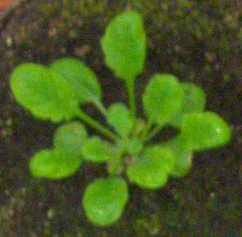
\includegraphics[width=0.25\textwidth]{ara2012_plant008_rgb}
  \caption{Example of Arabidopsis plant}
\end{figure}
\begin{figure}[h!]
  \centering
  \includegraphics[width=0.25\textwidth]{tobacco_plant034_rgb}
  \caption{Example of Tobacco plant}
\end{figure}
\subsection{Literature Review}
D.S.Guru et al. described a classification technique using \textit{K-nearest neighbour} (KNN) algorithm to classify flowers. \cite{guru2010texture} The author has used that method to classify different variants of flowers, which has inter-class variations and intra-class variations to be classified. This method is seriously considered due to the high similarities between the task mentioned in the paper prescribed and the task to be examined in this paper.\\

A.Salman et.al. described a method using \textit{Support Vector Machine} classifier to classify plants' leaves. They described this to be a very efficient method in distinguishing different plants leaves, which, in turn can be used in this paper.\cite{8068597}\\

S. Haug et al. described a method using \textit{Random Forest} method to classify crop and weed which they have an average accuracy of 93.8\%. The accuracy is high, hence it can be in turn used in this paper.\cite{6835733}

\section{Methods}
Here we use the three methods already described in the literature review section.\\

Scikit-learn\cite{scikitle87:online} provides all three methods in their library. The methods can be ran in Python by importing the packages. The packages are imported by the following code:\\

\begin{verbatim}
from sklearn import neighbors, svm
from sklearn.ensemble import RandomForestClassifier
\end{verbatim}

After importing the code, the three aforementioned method can be implemented using their constructors. We split the data of arapidopsis and tobacco into a randomized test and randomly retrieve 20\% of the sample size for training the algorithms. If the size is greater than 20\%, then one of the algorithms will have a 100\% accuracy, suggesting that there are too many samples to train the algorithms and a waste of resource.

\section{Experiment}

We run the source code in Python. We import some metrics from Scikit-learn to measure the performance of all three algorithms. This is done by the following code.
\begin{verbatim}
from sklearn.metrics import recall_score,\
accuracy_score, roc_curve, auc
\end{verbatim}

This imports the \textit{precision, recall} and \textit{AUC} methods of measuring performance. The code prints all three metrics to stdout and display the \textit{ROC} curve, which will be attached, using \textit{matplotlib.pyplot}.\\
Then, we use \textit{OpenCV} to read all 227 images into an array and extract the \textit{SIFT} features from it.\cite{4590383}\\

We then create \textit{KNN, SVM} and \textit{Random Forest} models and then train it using the sample image and their provided classifications, which is 20\% of the total images.\\

The parameters are set as the default values defined by each model.
\section{Experiment Results}
\subsection{Summary}
After running the Python code, the outputs are copied to the standard output. We copy them in the table below:
\begin{table}[]
\begin{tabular}{llll}
Method/Accuracy/Metric & Precision  & Recall     & AUC    \\
KNN                    & 93.4066 \% & 89.0385 \% & 0.9878 \\
SVM                    & 91.2088 \% & 84.6154 \% & 0.9947 \\
Random Forest          & 91.7582 \% & 85.5769 \% & 0.9982
\end{tabular}
\end{table}
\subsection{ROC curves}
A copy of ROC curve screenshots can be found below:\\
\begin{figure}[h!]
  \centering
  \includegraphics[width=0.45\textwidth]{Figure_1}
  \caption{ROC curve for KNN algorithm}
\end{figure}
\begin{figure}[h!]
  \centering
  \includegraphics[width=0.45\textwidth]{Figure_2}
  \caption{ROC curve for SVM algorithm}
\end{figure}
\begin{figure}[h!]
  \centering
  \includegraphics[width=0.45\textwidth]{Figure_3}
  \caption{ROC curve for Random Forest algorithm}
\end{figure}
\subsection{Summary}
From the above, we can conclude all three algorithms can effectively separate arabidopsis from tobacco, even with a small sample size. We can also coknclude that \textit{KNN} has the highest precision of all algorithms but \textit{Random Forest} has the highest \textit{AUC}.

%---bibliography---%
\bibliography{Indiv_rep} 
\bibliographystyle{ieeetr}
\end{document}

